\documentclass[12pt,oneside,a4paper]{article}

\usepackage[backend=biber,style=numeric, sorting=none]{biblatex}
\usepackage{xcolor}
\usepackage{todonotes}
\usepackage{amsmath}
\usepackage{multicol}
\usepackage{caption}
\usepackage{hyperref}
\usepackage{graphicx}
\usepackage{listings}
\usepackage[margin=1.35in]{geometry}

\lstdefinestyle{bsvstyle}{
	backgroundcolor=\color{backcolour},   
	numberstyle=\tiny\color{gray},
	basicstyle=\ttfamily\footnotesize,
	breakatwhitespace=false,         
	breaklines=true,                 
	captionpos=b,                    
	keepspaces=true,                 
	numbers=left,                    
	numbersep=5pt,                  
	showspaces=false,                
	showstringspaces=false,
	showtabs=false,                  
	tabsize=2
}

\lstdefinelanguage{BSV}{
	keywords={rule, Vector, int, String, Reg, Bit, begin, end, endrule, method, endmethod, Action, interface, endinterface, module, endmodule, Reg\#, Bool, let, True, False},
	keywordstyle=\color{codeblue}\bfseries,
	ndkeywords={import, if, else, return, deriving},
	ndkeywordstyle=\color{codepurple}\bfseries,
	identifierstyle=\color{black},
	sensitive=false,
	comment=[l]{//},
	morecomment=[s]{/*}{*/},
	commentstyle=\color{codegreen}\ttfamily,
	stringstyle=\color{red}\ttfamily,
	morestring=[b]',
	morestring=[b]"
}

\definecolor{codegreen}{RGB}{14, 161, 70}
\definecolor{codeblue}{RGB}{43, 45, 179}
\definecolor{codepurple}{RGB}{196, 53, 178}
\definecolor{backcolour}{RGB}{217, 217, 217}

\lstset{
	language=BSV,
	style=bsvstyle
}

\DeclareCaptionFormat{listing}{\rule{\dimexpr\textwidth\relax}{0.4pt}\par\vskip1pt#1#2#3}
\captionsetup[lstlisting]{format=listing,singlelinecheck=false, margin=0pt,labelsep=space,labelfont=bf}

\usepackage{booktabs}
\usepackage[noabbrev,capitalise]{cleveref}
\crefname{listing}{snippet}{snippet}
\Crefname{listing}{Algorithm}{Algorithms}
\renewcommand\lstlistingname{Code snippet}
\def\lstlistingcrefname{snippet}
\usepackage{url}

\addbibresource{biblio.bib}

\title{\textbf{RISC-V processors with Bluespec}}

\author{High Performance Processors and System\\ A.Y. 2020/2021\\\\\\\\\textbf{Riccardo Nannini}\\\\\\}

\date{\parbox{\linewidth}{\centering%
		\today\endgraf\bigskip\bigskip\bigskip\bigskip\bigskip
		Tutors: Emanuele Del Sozzo, \endgraf\medskip
		Davide Conficconi \endgraf\bigskip\bigskip
		Professor: Marco Domenico Santambrogio 
		}}
\begin{document}

\begin{titlepage}
	\centering
	\clearpage
	\maketitle
	\thispagestyle{empty}
	\vspace*{1cm}
	\vfill
	\centering
	
\includegraphics{logo_polimi.png}
\includegraphics{logo_NECST.png}
\end{titlepage}

\tableofcontents
\newpage

\begin{abstract}
Bluespec System Verilog (\textbf{BSV}) is a state-of-the-art Hardware Description Language.
Bluespec compilation toolchain (\textbf{BSC}) has been recently released as open source \cite{bsc}. The goal of the project was investigating the potentiality of said toolchain implementing different \textbf{RISC-V} processors of increasing complexity.\\
\end{abstract}

\section{Introduction} \label{sec:intro}

This report covers chronologically the path that I have followed during the development of this project.
 
It starts from a quick overview on the \textit{RISC-V} ISA, focused on the key ingredients that make this ISA one of the most trend topics in Computer Engineering.

It proceeds with the analysis of the \textit{Bluespec System Verilog} language, outlining its novelties with respect to other hardware description languages, as well as its main features and capabilities. 

The last section is devoted to the development of various RISC-V processor designs, describing in details the characteristics of each processor and motivating the various design choices, starting from a one cycle non pipelined processor and ending with a 6 stage pipelined one enriched with multiple branch predictors.

Everything I have produced within this project (code, scripts, this report itself) is available on GitHub \url{https://github.com/riccardo-nannini/BSV_RISC-V}


\section{RISC-V} \label{sec:risc-v}
\subsection{What is RISC-V}
Since the processor designs will be based on RISC-V, knowing this ISA is fundamental.

RISC-V was born in 2010 at UC Berkley by the work of graduate students Andrew Waterman, Yunsup Lee and professors David Patterson, Krste Asanovic \cite{risc-v_original}, built on the experience gained from the 4 previous major RISC ISA design from UC Berkeley (thus justifying the ‘V’).

As the name suggests, RISC-V belongs to the family of \textbf{RISC} ISAs. In particular, RISC instruction sets are characterized by \textit{small} and \textit{highly optimized} instructions that ease \textit{pipeline} implementation, along with a large number of \textit{general purpose registers}. 

RISC-V, like many other RISC ISAs, is a \textbf{load-store architecture}; this means that, apart from some exceptions, arithmetic and logic instructions operate on register and not on memory directly. Load and store instructions take care of the transit of data from memory to register and vice versa.
\subsection{Instructions set goals}
When the first paper that declared the birth of RISC-V \cite{risc-v_original} was released back in 2011, the authors stated some of the goals that they wanted to achieve when designing this instructions set. In particular the main objectives include, but are not limited to:
\begin{itemize}
	\item Provide a \textit{realistic} but \textit{open} ISA, suitable for direct hardware implementation
	\item Provide a \textbf{small} but \textbf{complete} ISA, that avoids "\textit{over-architecting}" for a particular microarchitecture style or implementation technology.
	\item Support highly-parallel multicore implementations, including heterogeneous multiprocessors
	\item Support an efficient dense \textit{instruction encoding} with variable-length instructions (generally typical of CISC ISAs).
	\item \textbf{base-plus-extension}: provide a set of standard but optional extensions.
\end{itemize}
In order to achieve these goals many design choices were taken, sometimes in line with other similar ISAs, sometimes with unusual decisions.

\subsection{Main features}
RISC-V has 2 base variants, \textbf{RV32} and \textbf{RV64}, providing 32-bit or 64-bit user-level address spaces respectively. A 128-bit extension is available but mostly aimed at the future of warehouse scale computing.
\subsubsection{Registers}
RISC-V uses 31 general-purpose registers  {\fontfamily{cmtt}\selectfont{x1-x31}} with  {\fontfamily{cmtt}\selectfont{x0}} hardwired to the costant 0. Moreover, 32 64-bit registers {\fontfamily{cmtt}\selectfont{f0-f31}} holding single or double-precision floating-point values are available.

There are also two special registers: the \textit{program counter} {\fontfamily{cmtt}\selectfont{pc}} holds the address of the current instruction while the \textit{floating point status register} {\fontfamily{cmtt}\selectfont{fsr}} contains the operating mode and exception status of the floating-point unit.
\subsubsection{Instruction encoding}
In addition to standard fixed-length 32-bit instructions, RISC-V supports extensions with \textbf{variable-length} ones too, useful in reducing code size specially for specific domains like embedded systems.

\cref{riscv:encoding} shows the instruction length encoding convention. 32-bit instructions have the 2 least significant bits always set to {\fontfamily{cmtt}\selectfont{1}} while the 16-bit ones must have said bits in any combination but {\fontfamily{cmtt}\selectfont{11}}.
Instructions longer than 32-bits have additional lower bits set to {\fontfamily{cmtt}\selectfont{1}}.\medskip

\begin{figure}[h]
	\centering
	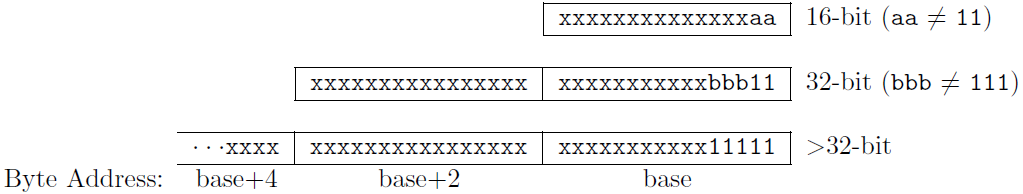
\includegraphics[scale=0.65]{risc-v_encoding}
	\caption{RISC-V instruction encoding}
	\label{riscv:encoding}
\end{figure}

\subsubsection{Instruction format}
Six basic instruction formats are present in the base version of the ISA as shown in \cref{riscv:format}.

\begin{figure}[h]
	\centering
	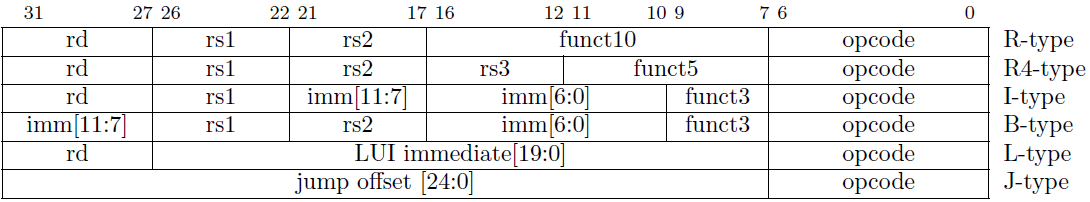
\includegraphics[scale=0.65]{risc-v_format}
	\caption{RISC-V instruction formats}
	\label{riscv:format}
\end{figure}

It is worth noting a particular design choice made by the authors. Since, as they state, the \textit{decoding} of register specifiers is usually on the \textbf{critical path} in implementations, they decided to keep all register specifiers in the same position across every instruction type. This comes with the tradeoff of having some instructions with an immediate value that has to be split in two parts.

\textbf{R-Type} instructions are for operations with two source registers (\textit{rs1} and \textit{rs2}) while \textbf{R4-Type} format is for special three source register floating point instructions. Moreover, \textbf{I-Type} format is for operations between a source register (\textit{rs1}) and an 12-bit sign-extended immediate, while \textbf{B-Type} instructions are designed for conditional branches (where the branch type is specified in \textit{funct3}).
The LUI (\textit{Load upper immediate}) operation, generally used to build 32-bit constants, is the typical instruction specified by the \textbf{L-Type}, meanwhile \textbf{J-Type} instructions encode a 25-bit target address as a PC-relative offset.

Describing in details the specification of every instruction is way out of the focus of this report and is already done with great details in the original paper \cite{risc-v_original}.\\

In the end, just a mention to the \textit{fsr}, a special register containing the status of floating-point operation, shown in \cref{riscv:fsr}.

\begin{figure}[h]
	\centering
	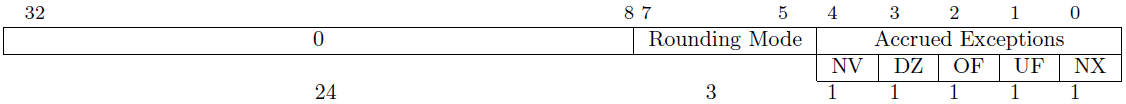
\includegraphics[scale=0.575]{risc-v_fsr}
	\caption{Floating-point status register}
	\label{riscv:fsr}
\end{figure}

It makes possible to specify the rounding mode with a specific encoding as well as reading the status of the previous floating-point operation in the flag bits.\\
\subsection{License}
Until here the main features of RISC-V were summarized.
Despite being a really well designed standard, this by itself does not explain the popularity of this ISA.

In fact, one of the main factor of his success is that RISC-V is provided under a \textbf{free open source} license that does not require fees to use.

This is quite unusual in the instruction set architectures world, that for a great majority are \textit{proprietary} due to historical or business reasons. Companies like ARM, IBM and Intel have patents on their ISAs which prevent others from using them without licenses.

Negotiations for said licenses can take 6-24 months and can cost up to \$1M-\$10M, ruling out academia and other with small volumes. An ARM license, for instance, doesn't even let you design an ARM core; you just get to you \textit{their} designs \cite{risc-v_free}.

Some open-source ISA already existed but were not as popular and well designed as RISC-V is.

The birth of this standard enabled a \textbf{real free open market} of processor designs leading to:
\begin{itemize}
	\item greater innovation via \textbf{free-market competition}
	\item shared open core designs
	\item processors becoming \textbf{affordable} for more devices
\end{itemize}

\section{BSV}
The hardware description language used to implement the RISC-V processor is \textbf{Bluespec System Verilog} (BSV).

Belonging to Bluespec Inc, co-founded in 2003 by MIT professor Arvind, the BSV language is aimed at providing hardware designers used to Verilog, VHDL or System Verilog, a \textbf{high level} language for hardware design and synthesis.

Based on a synthesizable subset of SystemVerilog, BSV can significantly improve the hardware design process with some key innovations: 

\begin{itemize}
	\item Hardware behavior is expressed with \textbf{Rules}.
	Rules are powerful concepts for achieving correct concurrency and eliminating race conditions.
	\item \textbf{Polymorphism} makes possible to write more general code and reuse designs and glue them together in a flexible way.
	\item Provides \textbf{formal semantics}, enabling formal verification and formal design-by-refinement. This is due to the fact that BSV rules are based on \textit{Term Rewriting Systems}, a clean formalism supported by decades of theoretical research in the computer science community.
\end{itemize}

\subsection{General overview}

This section is devoted to the main features of BSV in order to give the reader a general overview of the language and understand its strength. The complete reference guide (also used for this quick introduction) can be found at \cite{bsv_guide}.
\subsubsection{Modules and interfaces}
In order to understand BSV, it is useful start with the notion of \textbf{modules} and \textbf{interfaces}, the core of the language. Modules and interfaces are what, in the end, is turned into actual hardware. 

An interface describes what a module 'offers' to the outside. On the other hand, a module 'implements' its interface as it prefers.

In BSV, an interface consists of \textit{methods} that encapsulate the possible transactions that clients can perform. 

\begin{lstlisting}[label={list:moduleinterface},caption={Example of module and interface}]
interface Fifo#(int n);	//n is the size of the fifo

	method Action enqueue(Bool x);
	method Action dequeue;
	method Bit#(8) first;
	
endinterface

module mkFifo( Fifo#(n) );

	//... implementation
	
endmodule
\end{lstlisting}

When it comes to modules, however, we need to distinguish between a module \textit{definition} and a module \textit{instantiation}. A module definition is like a class in object oriented programming while a module instantation can be considered as an object of said class.

A module consists of three things: 
\begin{itemize}
	\item a \textbf{state}
	\item  \textbf{rules} that operate on that state
	\item an \textbf{interface} to the outside world
\end{itemize}
\subsubsection{State}
In Verilog and SystemVerilog, one simply declares a variable, and a synthesis tool "infers" how those variable actually map into state element in hardware; a variable may map into a bus, a latch, a flip-flop or even nothing.

BSV eliminates this ambiguity and places the state control directly in the hand of the designer. BSV \textit{never} implies state; variables are just convenient names for intermediate values.

State components are declared (and instantiated) after the module declaration like in \cref{bsv:state}

\begin{lstlisting}[label={bsv:state},caption={Example of state declaration}]
module mkFifo( Fifo#(n) );

    Vector#(n, Reg#(Bit#(8))) data <- replicateM(mkRegU());
		Reg#(Bit#(8)) 	  	 value_reg <- mkReg(0);
		
		//...

endmodule
\end{lstlisting}

\subsubsection{Types and polymorphism}

Every variable and every expression in BSV has a \textit{type}.
BSV supports standard \textit{simple type} like in \cref{bsv:simpletype}
\begin{lstlisting}[label={bsv:simpletype},caption={Simple types}]
int
Bool
String
\end{lstlisting}
or \textit{parametrized} types (either standard or user-defined)in the form of {\fontfamily{cmtt}\selectfont{\textbf{X\#}}(t\textsubscript{1},..., t\textsubscript{n})}
\begin{lstlisting}[label={bsv:paramtype},caption={Parametrized types}]
Typle2#(int, Bool)		//pair of items, an int and a Bool
List#(Bool)					  //list of booleans
Vector#(n, int)				//vector of n integers
Bit#(16)							//16-bit wide bit-vector
Int#(29)							//signed integer, 29 bits wide
Vector#(16, List#(Int#(29)))	//vector of 16 Lists of 29 bits wide signed integers
\end{lstlisting}

In \cref{bsv:paramtype} it is possible to observe that parametrized types utilize \textbf{polymorphism}, making code way more reusable.

It is worth mentioning also the type \textbf{Action} that denotes any expression that acts on the \textit{state} of the circuit, fundamental in order to produce useful hardware.
\subsubsection{Rules}
\textit{Rules} specity the internal behavior of modules. A rule may have a \textit{guard} (boolean expression) that indicates when the rule can execute (fire), and a \textit{body}, of type Action, that describes what the rule does.
\begin{lstlisting}[label={bsv:paramtype},caption={Autoincrementing couter with a single rule}]
module mkCounter(Empty);
	Reg#(Bit#(8)) value <- mkReg(0);
	
	rule increment (value >= 0); //guard
		value <= value + 1;			 	 //body
	endrule
endmodule
\end{lstlisting}

The body of a rule can contain, with an ad-hoc semantic, the basic constructs typical of software programming languages such as if-else, switch, loop etc.

\subsubsection{Dynamic semantic}

The simplest way to understand the dynamic semantic of BSV is thinking that, at each step, the system picks any \textit{one} enabled rule and fires it.

Since only one rule is executed at each step, we have only to look at each rule in \textbf{isolation}, without worrying about the interactions with other rules simultaneously. Each rule can be viewed as an \textbf{atomic state transition}.

The BSC compiler maps BSV into efficient parallel clocked synchronous hardware. In particular, the mapping allows multiple rules to be executed at each clock cycle. The compiler is able do to this by producing a \textbf{role-control circuit} which takes all the enabled conditions and possible data outputs (actions) and feeds them into a \textbf{scheduler} circuit. It is the scheduler duty, at each clock cycle, to select a subset of conflict-free rules to fire.

\section{Processor designs}
\newpage
\printbibliography

\end{document}


